\section*{5. \& 8. Bernoulli-Energy Methods}
\subsection*{5.1 General Procedure}
\begin{enumerate}
    \item There are 2 equations that are generally useful for these types of problems:
    \begin{enumerate}[label=\roman*)]
        \item Bernoulli's equation. Valid in regions of steady, incompressible 
        flow where net frictional forces are negligible.
        \item Mass flow rate: $\dot{m} = \rho A \dot{x} = \rho V$
    \end{enumerate}
    \item Identify the assumptions so the appropriate equations can be used.
    \item Try and cancel out as many terms as possible from the Bernoulli equation. Use mass flow rate to determine $\dot{x}$.
    \item Use energy methods to determine the pressure head if necessary.
\end{enumerate}
\subsection*{5.2 Variable Definitions}
\begin{itemize}
    \item $P$: Pressure
    \item $\dot{x}$: Velocity
    \item $z$: Elevation
    \item $V$: Volume
    \item $C_d$: Discharge coefficient
    \item $\beta$: Ratio of throat diameter to pipe diameter $d/D$
\end{itemize}
\subsection*{5.3 Formulas}
Classic Bernoulli Equations:
\begin{fleqn}
    \begin{align*}
        &\text{Bernoulli's Equation: } \frac{P_1}{\rho} + \frac{\dot{x}_1^2}{2} + gz_1 = \frac{P_2}{\rho} + \frac{\dot{x}_2^2}{2} + gz_2 \\
        &\text{Mass Conservation: } \Delta m_{\text{CV}} = \dot{m}_{\text{in}} - \dot{m}_{\text{out}} \\
        &\text{Mass Flow Rate: } \dot{m} = \rho A \dot{x} = \rho V \\
    \end{align*}
\end{fleqn}
Obstruction flowmeter:
\begin{figure}[H]
    \centering
    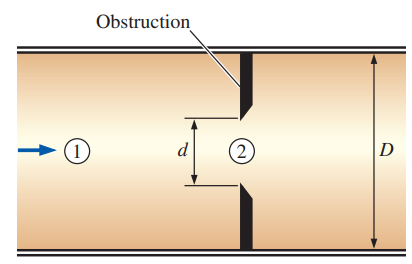
\includegraphics[width=0.2\textwidth]{Figures/Sec8 Obstruction Flowmeter.png}
    \caption{Obstruction flowmeter}
    \label{fig:obstruction_flowmeter}
\end{figure}
\begin{fleqn}
    \begin{align*}
        &\text{Obstruction flowmeter: } \dot{V} = A_0 C_d \sqrt{\frac{2(P_1 - P_2)}{\rho (1 - \beta^4)}} \\
        &\text{Mass Balance : } \implies \dot{x}_1 = (d/D)^2 \dot{x}_2 \\
        &\text{Head Loss: } h_L = \frac{P_1}{\rho g} + \frac{\dot{x}_1^2}{2g} + z_1 - \frac{P_2}{\rho g} - \frac{\dot{x}_2^2}{2g} - z_2 \\
    \end{align*}
\end{fleqn}